\chapter{Implementacija i korisničko sučelje}
		
		
		\section{Korištene tehnologije i alati}
		
			%\textbf{\textit{dio 2. revizije}}
			Kako bi što više ubrzali i olakšali komunikaciju među članovima tima, koristili smo dvije aplikacije: \underline{Whatsapp}\footnote{\url{https://www.whatsapp.com/}} i \underline{Discord}\footnote{\url{https://discord.com/}}. Kako bismo se dodatno upoznali s tehnologijom koja se često koristi u praksi, koristili smo i platformu \underline{Jira}\footnote{\url{https://www.atlassian.com/software/jira}} za organizaciju i podjelu zadataka na članove tima putem zadataka (engl. task) na Kanban ploči. Kao distribuirani sustav za upravljanje izvornim kodom koristili smo \underline{Git}\footnote{\url{https://git-scm.com/}}, a sami repozitorij projekta dostupan je na platformi \underline{Gitlab}\footnote{\url{https://gitlab.com/}}\\

            Za razvoj korisničkog sučelja tj. frontenda općenito, korišteni su markup jezik \underline{HTML}\footnote{\url{https://en.wikipedia.org/wiki/HTML}}, stilski jezik \underline{CSS}\footnote{\url{https://en.wikipedia.org/wiki/CSS}}, programski jezik \underline{Javascript}\footnote{\url{https://www.javascript.com/}} i \underline{React.js}\footnote{\url{https://reactjs.org/}}. React.js knjižnica je pisana u jeziku Javascript koja omogućava jednostavan i relativno brz razvoj komponenti koje je lako ponovno koristiti, a razvija ga primarno tvrtka Meta. Uz React.js, za razvoj robusnih i kvalitetnih komponenti, korišten je \underline{Material UI}\footnote{\url{https://mui.com/}} - open-source knjižnica React komponenti. Za pisanje koda u navedenim jezicima korišten je \underline{Visual Studio Code}\footnote{\url{https://code.visualstudio.com/}} - veoma popularan IDE (integrirana razvojna okolina) s velikim brojem opcionalnih ekstenzija koje služe kao pomoć pri razvoju. VSC razvija tvrtka Microsoft. \\

            \eject

            Za razvoj backenda korišten je programski jezik \underline{Java}\footnote{\url{https://www.java.com/en/}} - objektno orijentirani jezik korišten u brojnim aspektima razvoja programske potpore. Jezik Java razvija tvrtka Oracle. Uz to, korišten je \underline{Java Spring Boot}\footnote{\url{https://spring.io/projects/spring-boot}} - specijalizacija radnog okvira \underline{Java Spring}\footnote{\url{https://spring.io/}} razvijena s ciljem što bržeg, lakšeg i učinkovitijeg razvoja web aplikacija. Za pisanje koda u jeziku Java korišten je \underline{IntelliJ IDEA}\footnote{\url{https://www.jetbrains.com/idea/}} - integrirana razvojna okolina često korištena za razvoj programske potpore u jezicima Java i Kotlin. Intellij IDEA razvija tvrtka JetBrains. \\

            Za razvoj baze podataka korišten je sustav za upravljanje relacijskim bazama podataka \underline{PostgreSQL}\footnote{\url{https://www.postgresql.org/}}. Uz to, za lokalni razvoj i testiranje baze podataka korištena je aplikacija \underline{pgAdmin}\footnote{\url{https://www.pgadmin.org/}}. \\

            Za kreiranje potrebnih UML dijagrama korišten je alat \underline{Visual Paradigm Online}\footnote{\url{https://online.visual-paradigm.com/}} koji omogućava zajednički rad na dijagramima, time olakšavajući organizaciju i dijeljenje istih s članovima tima. Za razvoj dokumentacije korišten je markup jezik \underline{LaTeX}\footnote{\url{https://www.latex-project.org/}}, već navedena integrirana razvojna okolina Visual Studio Code i alat \underline{Overleaf}\footnote{\url{https://www.overleaf.com/}} koji omogućava online pisanje LaTeX koda.\\

            Frontend, backend i baza podataka pušteni su u pogon na platformi \underline{Render}\footnote{\url{https://render.com/}} koja omogućava besplatan i relativno jednostavan deploy aplikacija. Za uspješno puštanje u pogon backend koda, potrebno je pripremiti i \underline{Docker}\footnote{\url{https://www.docker.com/}} Container kako bi na istom mjestu bilo dostupno sve potrebno za uspješno puštanje backend-a u pogon. \\
		
			\eject 
		
	
		%\section{Ispitivanje programskog rješenja}
			
			%\textbf{\textit{dio 2. revizije}}\\
			
			 %\textit{U ovom poglavlju je potrebno opisati provedbu ispitivanja implementiranih funkcionalnosti na razini komponenti i na razini cijelog sustava s prikazom odabranih ispitnih slučajeva. 
			 %Studenti trebaju ispitati temeljnu funkcionalnost i rubne uvjete.}
	
			
			%\subsection{Ispitivanje komponenti}
			%\textit{Potrebno je provesti ispitivanje jedinica (engl. unit testing) nad razredima koji implementiraju temeljne funkcionalnosti. 
			%Razraditi \textbf{minimalno 6 ispitnih slučajeva} u kojima će se ispitati redovni slučajevi, rubni uvjeti te izazivanje pogreške (engl. exception throwing). 
			%Poželjno je stvoriti i ispitni slučaj koji koristi funkcionalnosti koje nisu implementirane. 
			%Potrebno je priložiti izvorni kôd svih ispitnih slučajeva te prikaz rezultata izvođenja ispita u razvojnom okruženju (prolaz/pad ispita). }
			
			
			
			%\subsection{Ispitivanje sustava}
			
			 %\textit{Potrebno je provesti i opisati ispitivanje sustava koristeći radni okvir Selenium\footnote{\url{https://www.seleniumhq.org/}}. 
			 %Razraditi \textbf{minimalno 4 ispitna slučaja} u kojima će se ispitati redovni slučajevi, 
			% rubni uvjeti te poziv funkcionalnosti koja nije implementirana/izaziva pogrešku kako bi se vidjelo na koji način sustav reagira kada nešto nije u potpunosti ostvareno. 
			 %Ispitni slučaj se treba sastojati od ulaza (npr. korisničko ime i lozinka), očekivanog izlaza ili rezultata, koraka ispitivanja i dobivenog izlaza ili rezultata.\\ }
			 
			 %\textit{Izradu ispitnih slučajeva pomoću radnog okvira Selenium moguće je provesti pomoću jednog od sljedeća dva alata:}
			 %\begin{itemize}
			 	%\item \textit{dodatak za preglednik \textbf{Selenium IDE} - snimanje korisnikovih akcija radi automatskog ponavljanja ispita	}
			 	%\item \textit{\textbf{Selenium WebDriver} - podrška za pisanje ispita u jezicima Java, C\#, PHP koristeći posebno programsko sučelje.}
			 %\end{itemize}
		 	%\textit{Detalji o korištenju alata Selenium bit će prikazani na posebnom predavanju tijekom semestra.}
			
			%\eject 
		
		
		\section{Dijagram razmještaja}
			
			%\textbf{\textit{dio 2. revizije}}

                Dijagram razmještaja opisuje konkretno ostvarenje odabrane arhitekture aplikacije - na slici 5.1 moguće je vidjeti raspodjelu programske potpore na konkretno sklopovlje. Kod za prikaz korisničkog sučelja i komunikaciju s korisnikom pisan u React.js pušten je u pogon na platformi Render. Kako bi aplikacija bila funkcionalna, u pogon su zasebno pušteni (engl. deployani) baza podataka ostvarena koristeći PostgreSQL te kod za poslovnu logiku i komunikaciju s bazom (backend) pisan u Java Spring Boot-u. Kako bi kod za backend bio uspješno deployan, za njega postoji i Docker container koji osigurava da je u njemu ispravno "spakiran" sav kod, kao i zavisnosti potrebne za uspješan rad istoga. I backend i baza podataka pušteni su u pogon koristeći platformu Render. \\

                Uz ovo, na platformi Firebase napravljen je Cloud Storage Bucket koji služi za jednostavnu pohranu slika potrebnih za uspješan prikaz oglasa. Komunikacija između zasebnih uređaja i platformi osigurana je protokolom HTTPS (komunikacija između klijentovog računala tj. web preglednika na istome i web poslužitelja deployanog na platformi Render, kao i komunikacija između web poslužitelja i Cloud Storage Bucket-a deployanog na platformi Firebase). Kako bi web poslužitelj korisniku mogao poslužiti sav potreban sadržaj, on komunicira s backendom koji po potrebi komunicira s bazom podataka.

                \begin{figure}[H]
				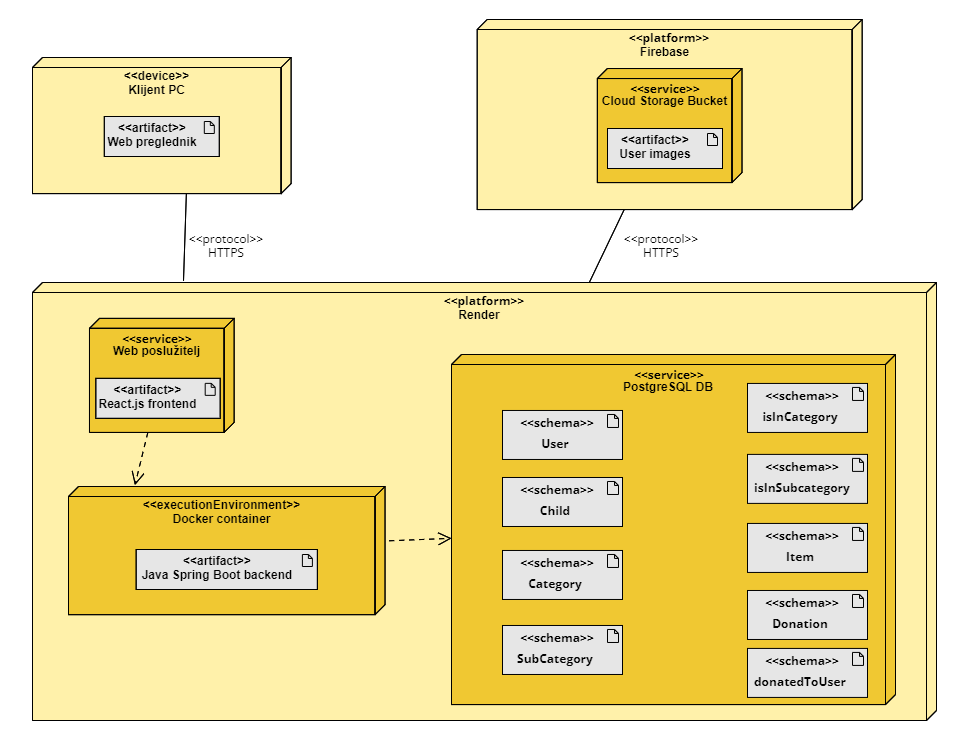
\includegraphics[width=\textwidth,height=0.8\textheight]{dijagrami/Dijagram razmjestaja.png}
				\centering
				\caption{Dijagram razmještaja}
				\label{fig:DeploymentDiagram}
			\end{figure}
			
			\eject 
		
		\section{Upute za puštanje u pogon}
		
			%\textbf{\textit{dio 2. revizije}}\\
                Frontend, backend i baza podatka puštene su u pogon na platformi Render. Upute za pristupanje platformi Render, kao i upute za puštanje u pogon (engl. deploy) slijede u sljedećim sekcijama.
          
			    \subsection{Pristupanje Renderu}

                Kako bi pristupili Renderu, prilikom prijave u web aplikaciju koristimo GitLab račune koji se direktno mogu povezati s njime. Povezivanjem Gitlab računa s platformom Render dobivamo lakši pristup kodu koji će se pustiti u pogon.

                \begin{figure}[H]
				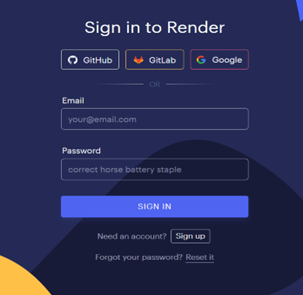
\includegraphics[width=0.6\textwidth,height=0.3\textheight]{slike/renderSignIn.png}
				\centering
				\caption{Render sign in}
				\label{fig:renderSignIn}
			\end{figure}

                \subsection{Backend deploy na Render}

                \textbf{1. Priprema}\\
                
                Prije puštanja aplikacije u pogon na Renderu potrebno je u izvorni kod za backend dodati Dockerfile za Maven projekt te u datoteci application.properties postaviti property server.servlet.context-path na /api da bude prefiks svim zahtjevima na backend.
			
			\eject 

                \textbf{2. Kreiranje baze podataka}\\

                U render dashboard potrebno je:

                \begin{itemize}
                    \item Pritisnuti tipku New te onda odabrati opciju PostgreSQL za kreiranje baze
                    \begin{figure}[H]
    			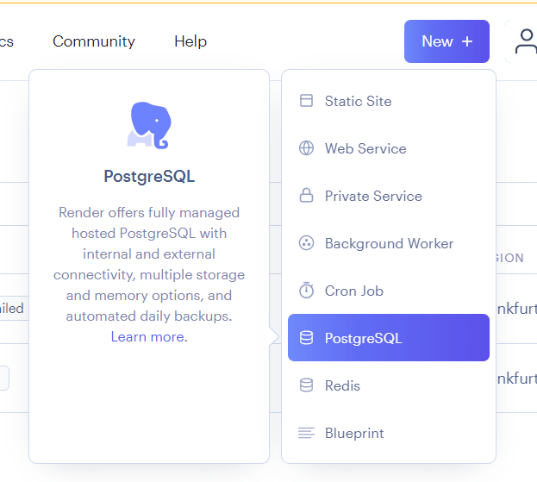
\includegraphics[width=0.6\textwidth,height=0.3\textheight]{slike/postgresqlCreate.png}
    			\centering
    			\caption{Kreiranje nove PostgreSQL baze}
    			\label{fig:newPostgreSQLDB}
    			\end{figure}
                    \item Postaviti ime baze
                    \item Database i User ostaviti prazno jer se automatski generira pri kreiranju baze
                    \item Postaviti Region na Frankfurt
                    \item Pritisnuti Create Database
                \end{itemize}

                \begin{figure}[H]
				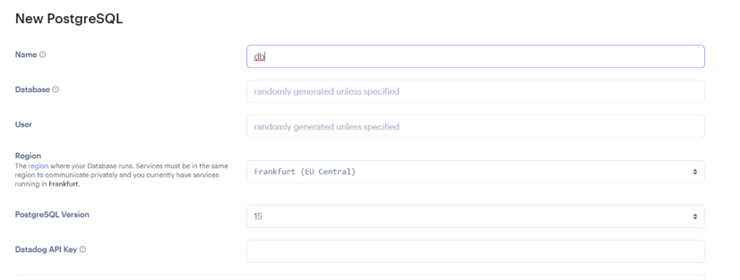
\includegraphics[width=0.8\textwidth,height=0.25\textheight]{slike/postgresqlNew.png}
				\centering
				\caption{Ispunjavanje podataka o bazi}
				\label{fig:postgresqlFillData}
			\end{figure}

                Prije puštanja backend-a u pogon, u datoteci application.properties moramo uvrstiti username, password za pristup bazi, database, hostname i port za url prema bazi na koju se treba spojiti.

                \begin{figure}[H]
				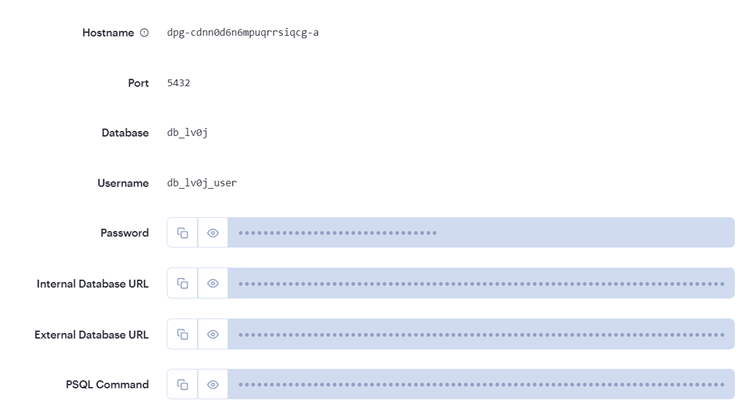
\includegraphics[width=0.8\textwidth,height=0.25\textheight]{slike/postgresqlNewFilled.png}
				\centering
				\caption{Ispunjavanje podataka u datoteci application.properties}
				\label{fig:applicationPropertiesDB}
			\end{figure}

                \textbf{3. Kreiranje backenda}\\

                U Render dashboard potrebno je:

                \begin{itemize}
                    \item Pritisnuti tipku New te onda odabrati opciju Web Service za kreiranje web usluge
                    \item Povezati GitLab račun - nakon povezivanja su za odabir dostupni svi projekti na koje imate prava pristupa
                    \item Pritisnuti Connect pokraj odgovarajućeg projekta
                    \begin{figure}[H]
    			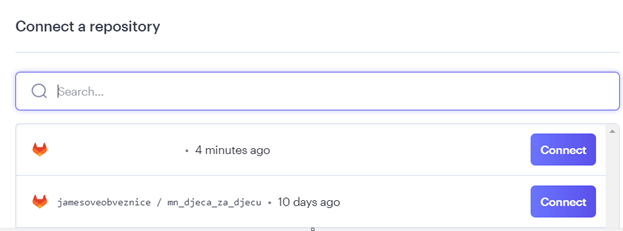
\includegraphics[width=0.8\textwidth,height=0.25\textheight]{slike/connectRepo.png}
    			\centering
    			\caption{Povezivanje repozitorija}
    			\label{fig:connectRepo}
    			\end{figure}
                    \item Postaviti ime za servis (ime servisa na kraju će biti dio web adrese)
                    \item Root directory postaviti na IzvorniKod/backend
                    \item Environment postaviti na Docker
                    \item Region postaviti na Frankfurt
                    \begin{figure}[H]
    			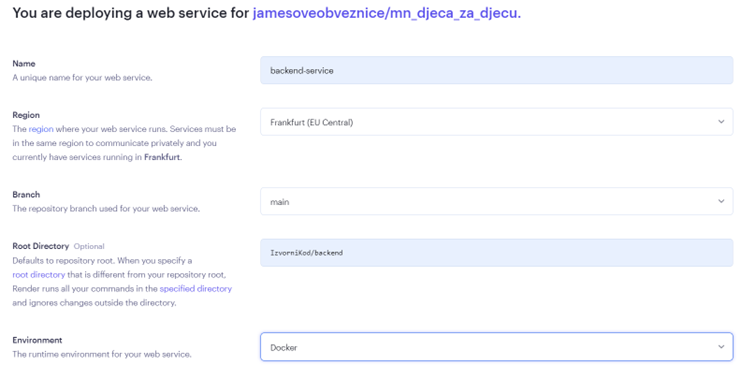
\includegraphics[width=0.8\textwidth,height=0.25\textheight]{slike/deployWebService.png}
    			\centering
    			\caption{Podaci za puštanje web servisa u pogon}
    			\label{fig:deployWebService}
    			\end{figure}
                    \item Na dnu proširiti \textit{advanced}
                    \item Postaviti putanju za Dockerfile ovisno koji se package manager koristi (u ovom slučaju putanja je ./docker/maven/Dockerfile)
                    \begin{figure}[H]
                    \makebox[\textwidth][c]{
\includegraphics[]{slike/dockerfilePath.png}}%
    			\centering
    			\caption{Putanja Dockerfile-a}
    			\label{fig:dockerFilePath}
    			\end{figure}
                    \item Pritisnuti Create Web Service
                \end{itemize}

                Nakon izvođenja svih ovih koraka, u pogon bi se trebala uspješno pustiti (eng. deployati) backend aplikacija. Nakon puštanja backend aplikacije u pogon, isto ćemo napraviti i za frontend aplikaciju.